\chapter{P and NP, SAT, Poly-time Reducibility}

\section{The Class of NP}

In a nondeterministic TM (NTM) decider, all branches halt on all inputs.
\begin{definition}
    An NTM \underline{runs in time} \(t(n)\) if all branches halt within \(t(n)\) steps on all inputs of length \(n\).  
    \begin{intuition}
        This is very strong constraint, this is because it should be able to \textit{verify} each branch in polynomial time. 
    \end{intuition}
\end{definition}

\begin{definition}
    \(NTIME(t(n)) = \{ B | \)some 1-tape NTM decides \(B\) and runs in time \(O(t(n))\)\}  

    \begin{figure}[H]
        \centering
        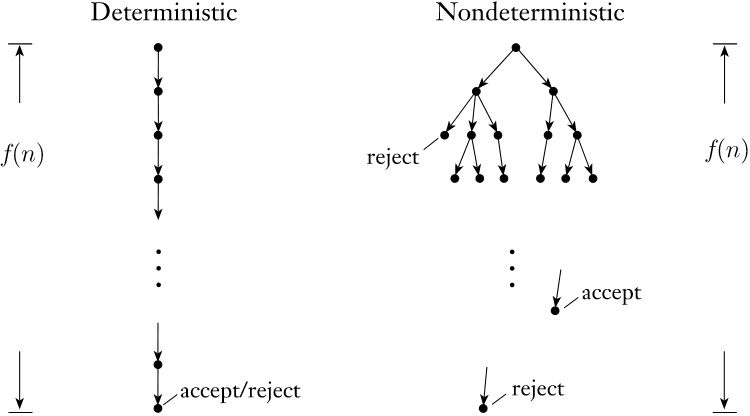
\includegraphics[width=0.7\textwidth]{f7.10.jpg}
        \caption{Comparing deterministic and nondeterministic time}
    \end{figure}
\end{definition}


\begin{definition}
    \(NP = \bigcup_k NTIME(n^k) = \) nondeterministic polynomial time decidable languages 
\end{definition}

\begin{itemize}
    \item Invariant for all reasonable nondeterministic models.
    \item Corresponds roughly to easily verifiable problems.
\end{itemize}

\section{Example of NP}
\begin{theorem}
    \(HAMPATH \in NP\) 
\end{theorem}
\begin{proof}
    We don't know if it's \(P\), but we can solve it in \(NP\).

    "On input \(\langle G, s, t \rangle\) (Say G has \(m\) nodes)
    \begin{enumerate}
        \item Nondeterministically write a sequence \(v_1, v_2, \cdots, v_m\) of \(m\) nodes
        \item Accept if 
        \(v_1 = s\) 

        \(v_m = t\)  
        
        each \(v_i, v_i+1\) is an edge
        
        and no \(v_i\) repeats
        \item Reject if any condition fails."
    \end{enumerate}

    \begin{remark}
        The mindset for this is that in step 1, we generate all possible sequence, this is neither \(P\) nor \(NP\), because it is not a decision problem. 

        Step 2, each branch/path/permutation/sequence can be verified in \(P\) time, and this can be checked by a nondeterministic machine. 
        That's the reason we say HAMPATH belongs to class \(NP\) languages. 
    \end{remark}
\end{proof}

\begin{definition}[COMPOSITES]
    \(COMPOSITES = \) 
    \{\(x|x\) is not prime and \(x\) is written in binary\} 

    = \{\(x|x = yz\) for int \(y, z > 1\), \(x\) in binary\}
\end{definition}

\begin{theorem}
    \(COMPOSITES \in NP \) 
\end{theorem}
\begin{proof}
    "On input \(x\) 
    \begin{enumerate}
        \item Nondeterministically write \(y\) where \(1 < y < x\)
        \item Accept if \(y\) divides \(x\) with remainder \(0\).    

        Reject if not."
    \end{enumerate}

    \begin{note}[2002]
    \(COMPOSITES \in P\) has been proved in 2002:

    \href{https://en.wikipedia.org/wiki/AKS_primality_test}{AKS primality test}
    \end{note}
\end{proof}

\section{P vs NP}

\begin{intuition}
    NP = All languages where you can \underline{verify} membership quickly (this is called \textbf{short certificates})

    P = All languages where can \underbar{test} membership quickly
\end{intuition}

We know that \(P \subseteq NP\), but \(P = NP\) (Cook 1971)? 

\begin{problem}
    Let \(\overline{HAMPATH}\) be the complement to \(HAMPATH\). 

    \(\langle G, s, t \rangle \in \overline{HAMPATH}\) if \(G\) does not have a HAMPATH path from \(s\) to \(t\).   

    Is \(\overline{HAMPATH} \in NP\)? 

    The reasonable answer is "We Don't Know". 

    Note that we cannot invert the accept/reject output of the NTM for it, this is not how nondeterministic works!!!
\end{problem}

\subsection{Dynamic Programming}
\begin{theorem}[Recall]
    \(A_{CFG}\) = \{\(\langle G, w \rangle | G\) is a CFG and \(w \in L(G)\) \} 

    \(A_{CFG}\) is decidable. 
\end{theorem}
\begin{proof}
    (Using \hyperref[theorem: Chomsky]{Chomsky Normal Form(CNF)}). This gave an NP type algorithm.
\end{proof}

\begin{theorem}
    \(A_{CFG} \in P\) 
\end{theorem}
\begin{proof}
    Recursive algorithm \(C\) tests if \(G\) generates \(w\), starting at any specified variable \(R\).    

    \(C\) = "On input \(\langle G, w, R \rangle\)
    \begin{enumerate}
        \item For each way to divide \(w = xy\) and for each rule \(R \rightarrow ST\)
        \item Use \(C\) to test \(\langle G, x, S \rangle\) and \(\langle G, y, T \rangle\) 
        \item Accept if both accept
        \item Reject if none of above accepted."    
    \end{enumerate}  
    Then decide \(A_{CFG}\) by starting from \(G\)'s start variable.  

    \(C\) is a correct algorithm, but it takes non-polynomial time. 

    \begin{remark}[Fix]
       Use recursion + memory called \(Dynamic Programming (DP)\)  
    \end{remark}

    Here's a fixed version:

    \(D\) = "On input \(\langle G, w, R \rangle\)
    \begin{enumerate}
        \item \textcolor{red}{If previously solved \(\langle G, w, R \rangle\) then answer same, else continue}. 
        \item For each way to divide \(w = xy\) and for each rule \(R \rightarrow ST\)
        \item Use \(D\) to test \(\langle G, x, S \rangle\) and \(\langle G, y, T \rangle\) 
        \item Accept if both accept
        \item Reject if none of above accepted."    
    \end{enumerate}  
    Then decide \(A_{CFG}\) by starting from \(G\)'s start variable.  
\end{proof}

\textbf{Bottom-Up DP} is also briefly discussed, which is the iterative way of DP, as we often see in algorithm courses.

\section{Satisfiability Problem}
\begin{definition}
    A \textbf{Boolean formula \(\phi\)}  has Boolean variables (TURE/FALSE values) and Boolean operations \verb|AND|(\(\land\)), \verb|OR|(\(\lor\)), and \verb|NOT|(\(\neg\)).
\end{definition}

\begin{definition}
    \(\phi\) is \textbf{satisfiable} if \(\phi\) evaluates to \verb|TRUE| for some assignment to its variables. 
\end{definition}

\begin{example}
    Let \(\phi = (x \lor y) \land (\bar{x} \lor \bar{y})\) (Notation: \(\bar{x}\) means \(\neg y\)). 
\end{example}

\begin{definition}
    \(SAT\) = \{ \(\langle \phi \rangle | \phi\) is satisfiable Boolean formula\} 
\end{definition}

\begin{definition}[Cook, Levin 1971]
    \(SAT \in P \implies P = NP\)  
\end{definition}
\begin{proof}
    polynomial time (mapping) reducibility (will be proved in later lecture). 
\end{proof}

\begin{remark}
        \(SAT \in NP\) (Obviously)
\end{remark}

\subsection{Polynomial Time Reducibility}
\begin{definition}
    \(A\) is \underline{polynomial time reducible} to \(B\) (\(A \leq_P B\))  if \(A \leq_m B\) by a reduction function \(f: \Sigma^* \mapsto \Sigma^*\) that is computable in polynomial time.

    For every \(w\):
    \[
        w \in A \iff f(w) \in B
    \]

    The function \(f\) is called \textbf{polynomial time reduction} of A to B.
\end{definition}
\begin{theorem}
    If \( A \leq_P B\) and \(B \in P\) then \(A \in P\). 
\end{theorem}
\begin{proof}
    \(A \leq_P B\): \(\forall w \in A\), we can find a function \(f\) making \(f(w) \in B\).    

    \(B \in P\): \(\forall w \in B\), there exists a TM \(M\) which can compute \(w\) in polynomial time.  

    To prove \(A \in P \implies\) there's a TM which can compute all strings in \(A\) at polynomial time.    

    \(N\) = "On input \(w\),
    \begin{enumerate}
        \item compute \(f(w)\).
        \item using TM \(M\) to decide \(f(w)\), return the result."     
    \end{enumerate}  

    If \(w \in A\), then \(f(w)\) in \(B\). 
    The above 2 steps are both polynomial, so \(N\) can decide \(w\) in polynomial time, 
    meaning \(A \in P\). 
\end{proof}

\begin{note}[Analog with \(A_{TM}\) ]
    All T-recognizable languages are polynomial reducible to \(A_{TM}\).   
\end{note}